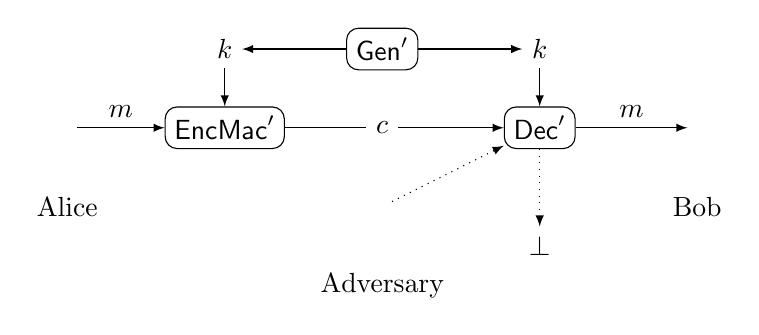
\begin{tikzpicture}
\node (sender) {\Alice};
\node (bart) [below of = sender] {Alice};
\node (enc) [draw, right of = sender, rounded corners=1ex,node distance = 2cm] {$\mathsf{EncMac}'$};
\node (k1) [above of = enc, node distance = 1cm] {$k$};
\node (c) [right of = enc, node distance = 2cm] {$c$};
\node (gen) [draw, above of = c, rounded corners=1ex,node distance = 1cm] {$\mathsf{Gen}'$};
\node (adv) [below of = c, node distance = 1cm] {\Adversary};
\node (burns) [below of = adv] {Adversary};
\node (dec) [draw, right of = c, rounded corners=1ex,node distance = 2cm] {$\mathsf{Dec}'$};
\node (k2) [above of = dec, node distance = 1cm] {$k$};
\node (receiver) [right of = dec, node distance = 2cm] {\Bob};
\node (lisa) [below of = receiver] {Bob};
\draw[-latex] (sender) -- (enc) node [midway, above] {$m$};
\draw (enc) -- (c); \draw[-latex] (c) -- (dec);
\draw[-latex] (dec) -- (receiver) node [midway, above] {$m$};
\draw[-latex] (k1) -- (enc);
\draw[-latex] (gen) -- (k1);
\draw[-latex] (gen) -- (k2);								
\draw[-latex] (k2) -- (dec);
\node (perp) [below of=dec, node distance = 1.5cm] {$\perp$};
\draw[dotted,-latex] (adv) -- (dec);
\draw[dotted,-latex] (dec) -- (perp);
\end{tikzpicture}